\documentclass{beamer}
\usepackage[latin1]{inputenc}
\usepackage{times}
\usepackage{tikz}
\usetheme{Luebeck}
%\usecolortheme{albatross}
\usepackage{amsmath,amsfonts,amsthm,amssymb}
\usepackage{setspace}
\usepackage{Tabbing}
\usepackage{fancyhdr}
\usepackage{lastpage}
\usepackage{extramarks}
\usepackage{chngpage}
\usepackage{soul,color}
\usepackage{graphicx,float,wrapfig}
\usepackage{xcolor}
\usepackage{listings}
\usepackage{float}
%\usepackage{subfloat}
\usepackage{subfigure}
\usepackage{caption}
\usepackage{enumitem}
\usepackage{algpseudocode}

\definecolor{darkorange}{RGB}{240, 120, 0}
\definecolor{darkgreen}{RGB}{0, 128, 0}
\definecolor{darkred}{RGB}{128, 0, 0}

\setbeamercolor{background canvas}{bg=white}
\setbeamercolor{frametitle}{fg=white, bg=darkorange}
\setbeamercolor{normal text}{bg=black,fg=black}
\setbeamercolor{structure}{bg=black, fg=darkorange}


\lstdefinestyle{customc}{
  belowcaptionskip=1\baselineskip,
  breaklines=true,
  frame=L,
  xleftmargin=\parindent,
  language=Python,
  showstringspaces=false,
  basicstyle=\footnotesize\ttfamily,
  keywordstyle=\bfseries\color{green!40!black},
  commentstyle=\itshape\color{purple!40!black},
  identifierstyle=\color{blue},
  stringstyle=\color{orange},
}

\lstdefinestyle{customc}{
  belowcaptionskip=1\baselineskip,
  breaklines=true,
  frame=L,
  xleftmargin=\parindent,
  language=Python,
  showstringspaces=false,
  basicstyle=\footnotesize\ttfamily,
  keywordstyle=\bfseries\color{green!40!black},
  commentstyle=\itshape\color{purple!40!black},
  identifierstyle=\color{blue},
  stringstyle=\color{orange},
}

\lstdefinestyle{customcsmall}{
  belowcaptionskip=1\baselineskip,
  breaklines=true,
  frame=L,
  xleftmargin=\parindent,
  language=Python,
  showstringspaces=false,
  basicstyle=\footnotesize\ttfamily,
  keywordstyle=\bfseries\color{green!24!black},
  commentstyle=\itshape\color{purple!24!black},
  identifierstyle=\color{blue},
  stringstyle=\color{orange},
}

\lstdefinestyle{customcsmall}{
  belowcaptionskip=1\baselineskip,
  breaklines=true,
  frame=L,
  xleftmargin=\parindent,
  language=Python,
  showstringspaces=false,
  basicstyle=\footnotesize\ttfamily,
  keywordstyle=\bfseries\color{green!24!black},
  commentstyle=\itshape\color{purple!24!black},
  identifierstyle=\color{blue},
  stringstyle=\color{orange},
}

\definecolor{MidGreen}{HTML}{00AA00}
\definecolor{MidYellow}{HTML}{AAAA00}

\title{Lecture 26: MDS / Canonical Forms}
\date{4/19/2016}
\institute{Chris Tralie, Duke University}
\author{COMPSCI/MATH 290-04}
\begin{document}

\frame{\titlepage}

\begin{frame}{Announcements}
\begin{itemize}[label=$\vartriangleright$]

\item Group Assignment 3 Final Deadline Tuesday 4/26

\item Guest Lecture Thursday

\item No office hours Thursday

\end{itemize}

\end{frame}


\begin{frame}{Spin Images}

Why did they all look so boring and unlike the objects in question?

\begin{figure}[t]
    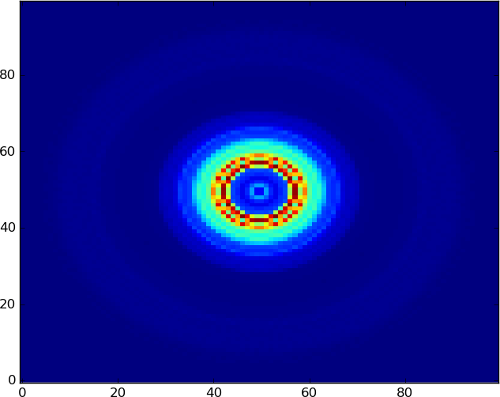
\includegraphics[width=0.7\textwidth]{SpinImage.png}
\end{figure}


\end{frame}

\begin{frame}{Spin Images}

\begin{figure}[t]
    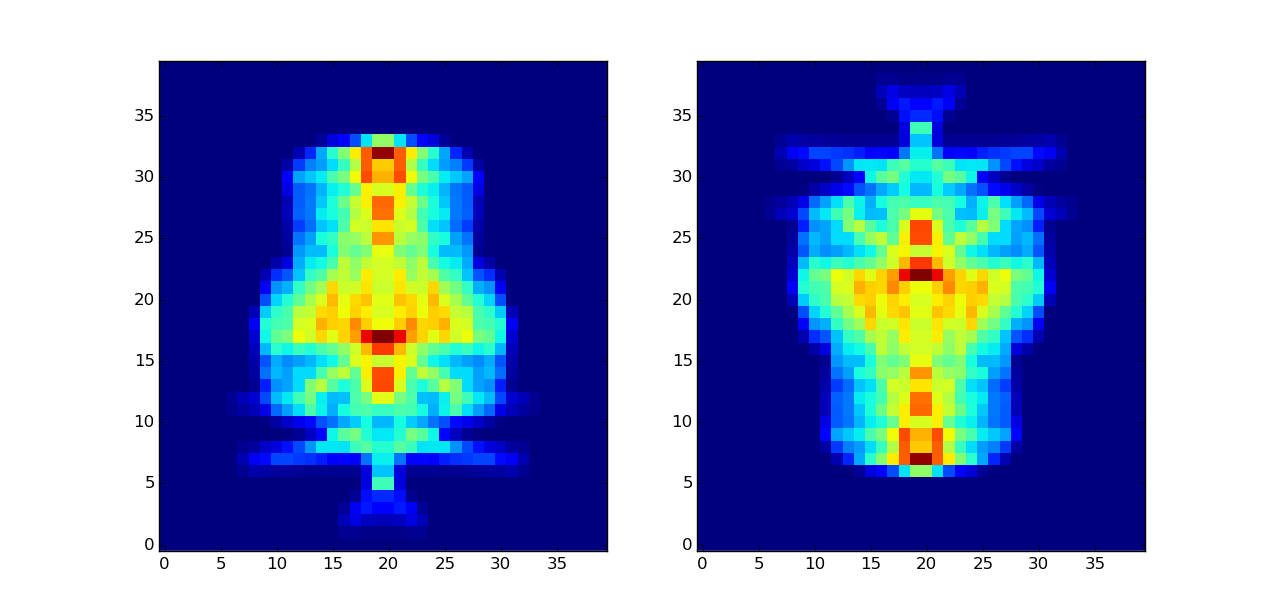
\includegraphics[width=\textwidth]{Hist12.png}
\end{figure}

I made a mistake on the assignment!  First principal axis is vertical axis in image

\end{frame}


\begin{frame}{Table of Contents}

\begin{itemize}[label=$\blacktriangleright$]
	\item Multidimensional Scaling
\end{itemize}

\begin{itemize}[label=$\vartriangleright$]
	\item Canonical Forms
\end{itemize}


\end{frame}

\begin{frame}{Academic Majors Distances: Your Choices}

\begin{figure}[t]
    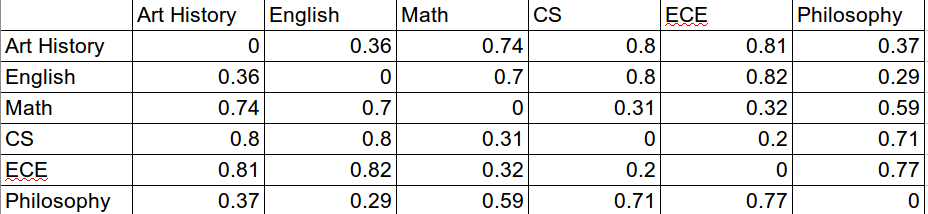
\includegraphics[width=0.7\textwidth]{ClassChoices.png}
\end{figure}
\small Multidimensional Scaling down to $\mathbb{R}^2$
\begin{figure}[t]
    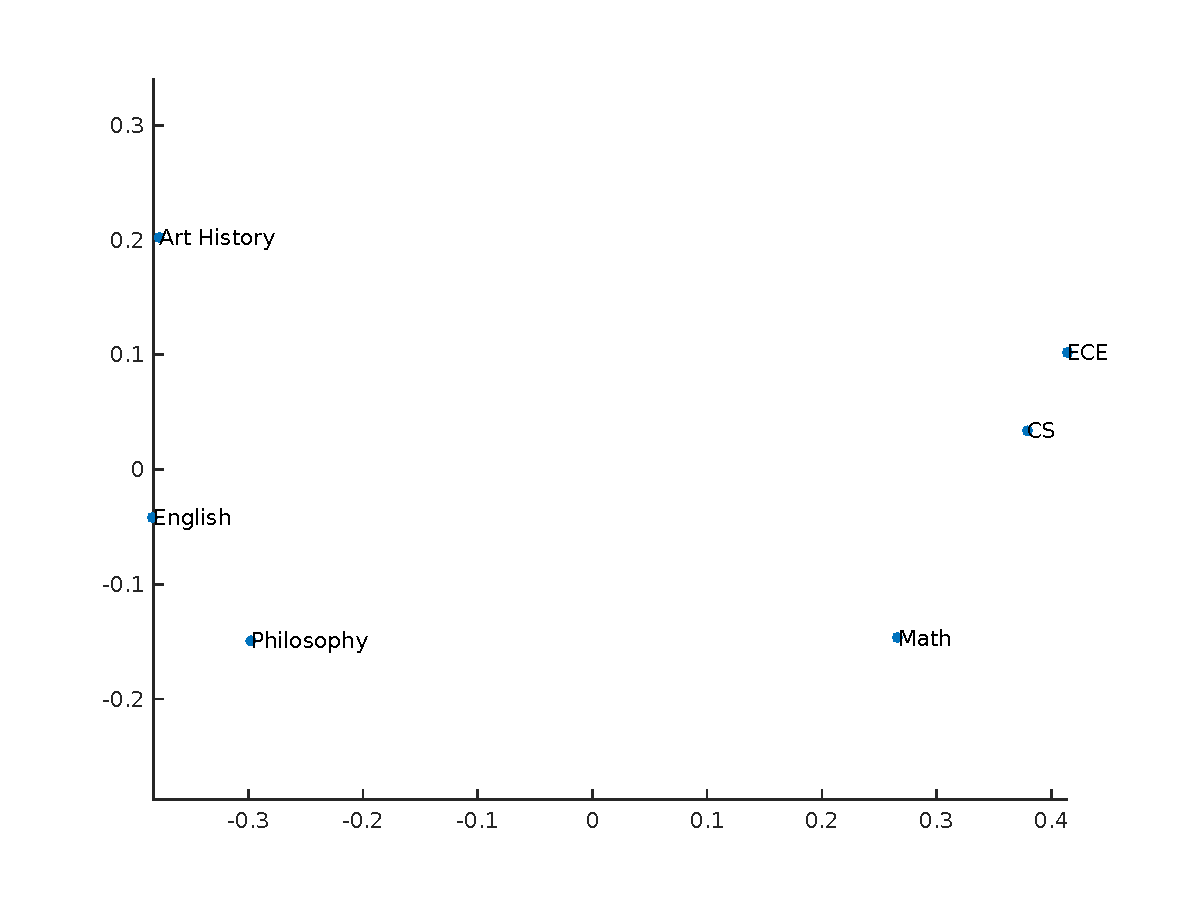
\includegraphics[width=0.65\textwidth]{MDSClasses.pdf}
\end{figure}


\end{frame}


\begin{frame}{Academic Majors Distances: Chris's Choices}

\begin{figure}[t]
    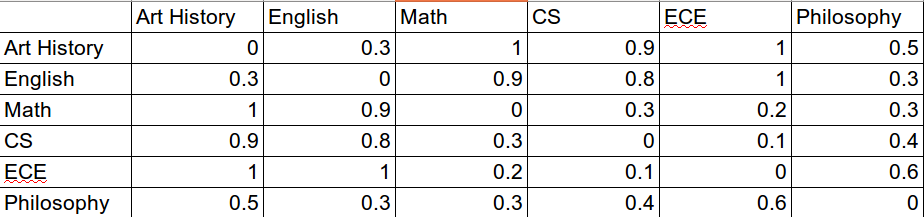
\includegraphics[width=0.7\textwidth]{ChrisChoices.png}
\end{figure}
\small Multidimensional Scaling down to $\mathbb{R}^2$
\begin{figure}[t]
    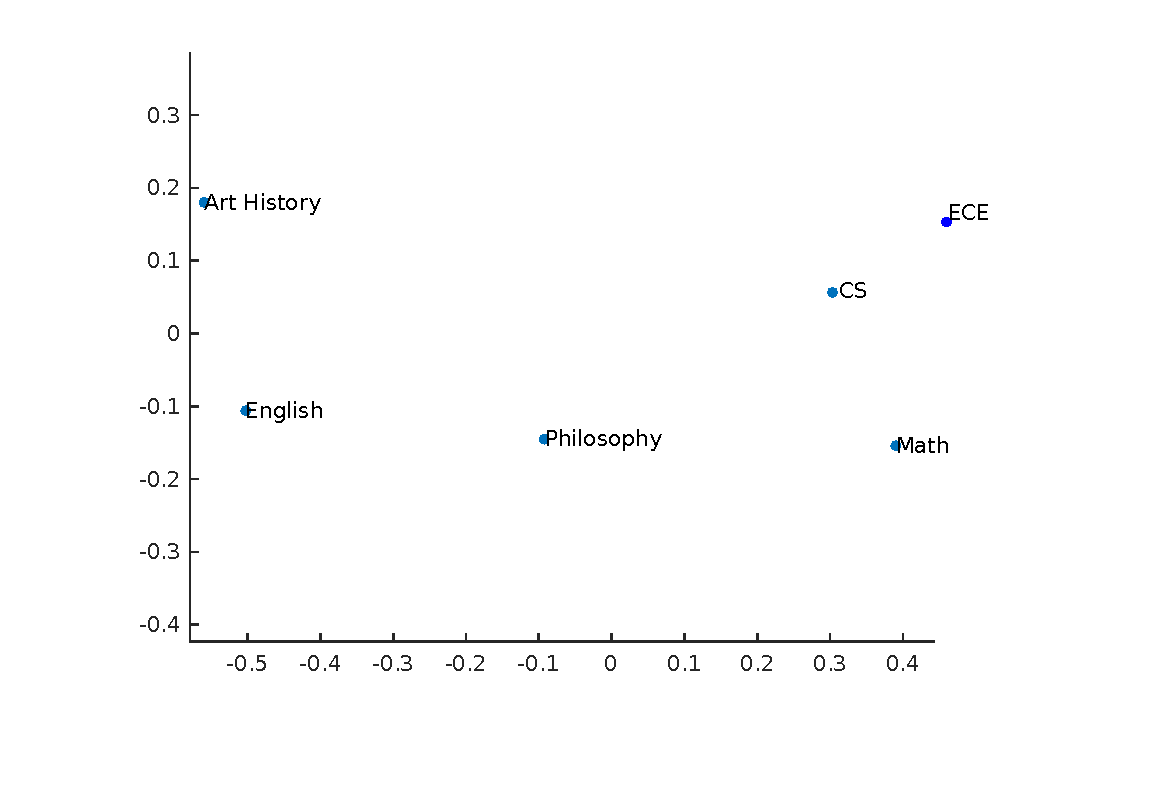
\includegraphics[width=0.65\textwidth]{MDSClasses_Chris.pdf}
\end{figure}


\end{frame}

\begin{frame}{Multidimensional Scaling}

\begin{itemize}[label=$\vartriangleright$]
\item Given an $N \times N$ symmetric discrete similarity matrix $D$ (i.e. $D_{ij} = D_{ji}$)
\item Given a Euclidean dimension $K$
\end{itemize}

Find a point cloud $X \in \mathbb{R}^{N \times K}$ so that

\[ D_{ij} \approx \sqrt{\sum_{k = 1}^K (X[i, k] - X[j, k])^2} \]

\uncover<2->{
In other words, find a point cloud in Euclidean $K$-space that {\em best approximates} the distances
}

\end{frame}

\begin{frame}{MDS: Euclidean Dimension Reduction}

\[ D_{ij} \approx \sqrt{\sum_{k = 1}^K (X[i, k] - X[j, k])^2} \]

What if $D_{ij}$ comes from a Euclidena space of dimension $d > k$?  Can we solve this using something else we learned in the course?

\uncover<2->{

This is equivalent to PCA!!  If we let $k = d$, then we can represent distances exactly

}

\end{frame}

\begin{frame}{MDS: Non-Euclidean Space Reduction}

Can we always find a point cloud that satisfies a given $D$ by making $k$ arbitrarily high?

\uncover<2->{
Assume sphere of radius $2/\pi$ with points in the following configuration:

\begin{columns}
\begin{column}[T]{4cm}
\begin{figure}[t]
    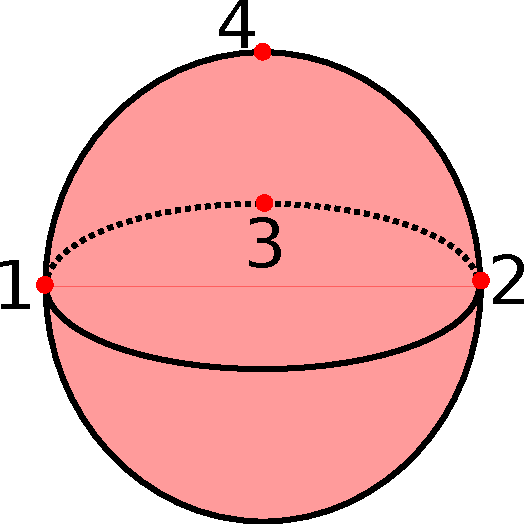
\includegraphics[width=\textwidth]{SphereLinial.pdf}
\end{figure}
\end{column}

\begin{column}[T]{4cm}
\begin{center}
  \begin{tabular}{ | l | c | c | c | r | }
     & $v_1$ & $v_2$ & $v_3$ & $v_4$ \\
    $v_1$ &      &      &      &      \\ \hline
    $v_2$ &      &      &      &      \\ \hline
    $v_3$ &      &      &      &      \\ \hline
    $v_4$ &      &      &      &     
  \end{tabular}
\end{center}
\end{column}
\end{columns}

}

\end{frame}


\begin{frame}{MDS: Non-Euclidean Space Reduction}

Can we always find a point cloud that satisfies a given $D$ by making $k$ arbitrarily high?

Assume sphere of radius $2/\pi$ with points in the following configuration:

\begin{columns}
\begin{column}[T]{4cm}
\begin{figure}[t]
    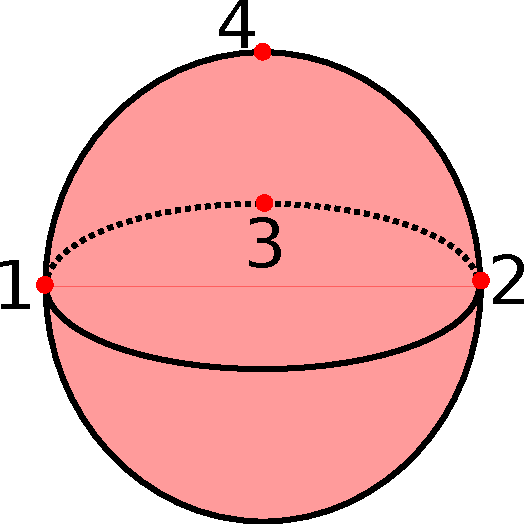
\includegraphics[width=\textwidth]{SphereLinial.pdf}
\end{figure}
\end{column}

\begin{column}[T]{4cm}
\begin{center}
  \begin{tabular}{ | l | c | c | c | r | }
     & $v_1$ & $v_2$ & $v_3$ & $v_4$ \\
    $v_1$ & 0 & 2 & 1 & 1 \\ \hline
    $v_2$ & 2 & 0 & 1 & 1 \\ \hline
    $v_3$ & 1 & 1 & 0 & 1 \\ \hline
    $v_4$ & 1 & 1 & 1 & 0
  \end{tabular}
\end{center}
\end{column}
\end{columns}

\end{frame}


\begin{frame}{MDS: Non-Euclidean Space Reduction}

Assume sphere of radius $2/\pi$ with points in the following configuration:

\begin{columns}
\begin{column}[T]{4cm}
\begin{figure}[t]
    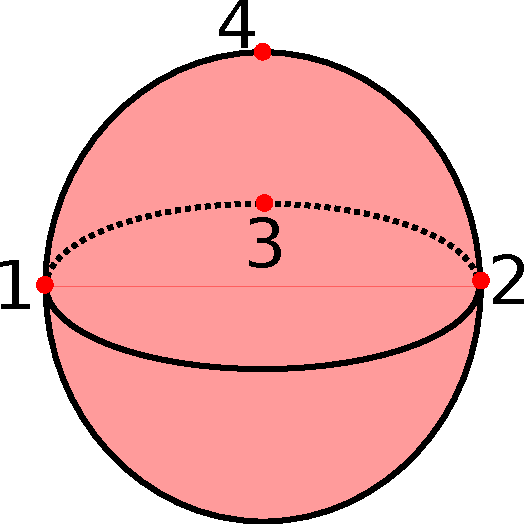
\includegraphics[width=0.7\textwidth]{SphereLinial.pdf}
\end{figure}
\end{column}

\begin{column}[T]{4cm}
\begin{center}
  \begin{tabular}{ | l | c | c | c | r | }
     & $v_1$ & $v_2$ & $v_3$ & $v_4$ \\
    $v_1$ & 0 & 2 & 1 & 1 \\ \hline
    $v_2$ & 2 & 0 & 1 & 1 \\ \hline
    $v_3$ & 1 & 1 & 0 & 1 \\ \hline
    $v_4$ & 1 & 1 & 1 & 0
  \end{tabular}
\end{center}
\end{column}
\end{columns}

\begin{columns}
\begin{column}[T]{4cm}
\uncover<2->{
\begin{figure}[t]
    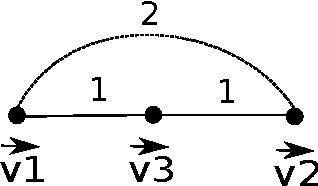
\includegraphics[width=0.6\textwidth]{PointsLineSphere1.pdf}
\end{figure}
$v_1,v_3,v_2$ along a line
}
\end{column}

\begin{column}[T]{4cm}
\begin{center}
\uncover<3->{
\begin{figure}[t]
    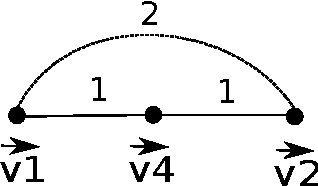
\includegraphics[width=0.6\textwidth]{PointsLineSphere2.pdf}
\end{figure}
$v_1,v_4,v_2$ also along line!
}
\end{center}
\end{column}
\end{columns}


\end{frame}


\begin{frame}{MDS: Non-Euclidean Space Reduction}

\begin{columns}
\begin{column}[T]{4cm}
\begin{figure}[t]
    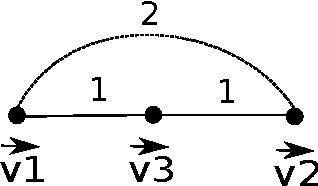
\includegraphics[width=0.6\textwidth]{PointsLineSphere1.pdf}
\end{figure}
$v_1,v_3,v_2$ along a line
\end{column}

\begin{column}[T]{4cm}
\begin{center}
\begin{figure}[t]
    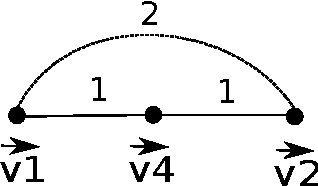
\includegraphics[width=0.6\textwidth]{PointsLineSphere2.pdf}
\end{figure}
$v_1,v_4,v_2$ also along line!
\end{center}
\end{column}
\end{columns}

This implies that $v_4$ and $v_3$ must collapse to the same point in any Euclidean space.

\begin{itemize}[label=$\vartriangleright$]
\item In other words, distances along the sphere cannot be perfectly realized using a Euclidean space of any finite dimension!
\uncover<2->{
\item (But let's do our best and see what we come up with)
}
\end{itemize}

\end{frame}

\begin{frame}{Table of Contents}

\begin{itemize}[label=$\blacktriangleright$]
	\item Multidimensional Scaling
\end{itemize}

\begin{itemize}[label=$\vartriangleright$]
	\item Canonical Forms
\end{itemize}

\end{frame}

\begin{frame}{Nonrigid Shape Alignment}

How do I align these two camels??

\begin{figure}[t]
    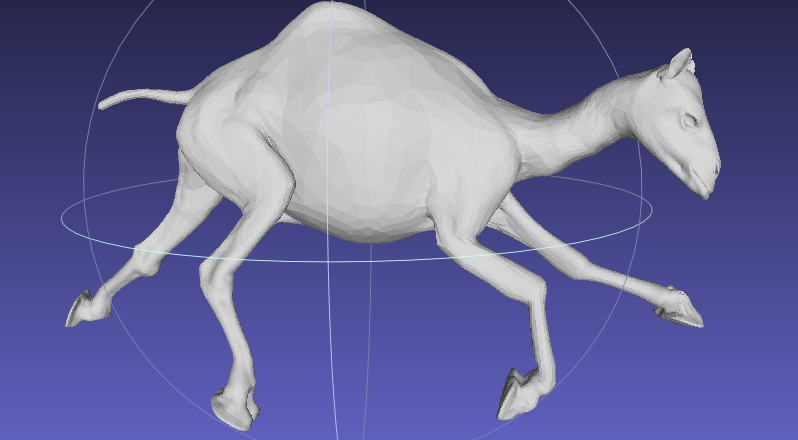
\includegraphics[width=0.45\textwidth]{camelpose1.png}
\end{figure}

\begin{figure}[t]
    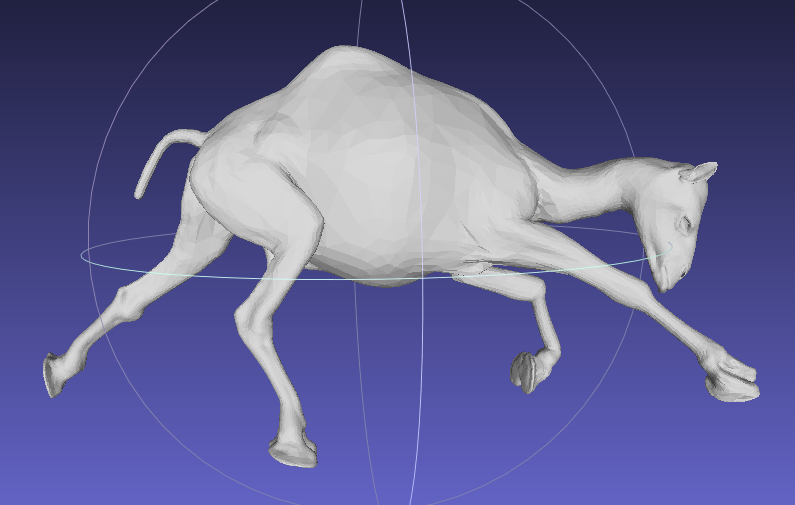
\includegraphics[width=0.4\textwidth]{camelpose2.png}
\end{figure}


\end{frame}

\begin{frame}{Geodesic Distances}

Geodesic distances are invariant to {\em isometries} (aka bending without stretching)
\begin{figure}[t]
    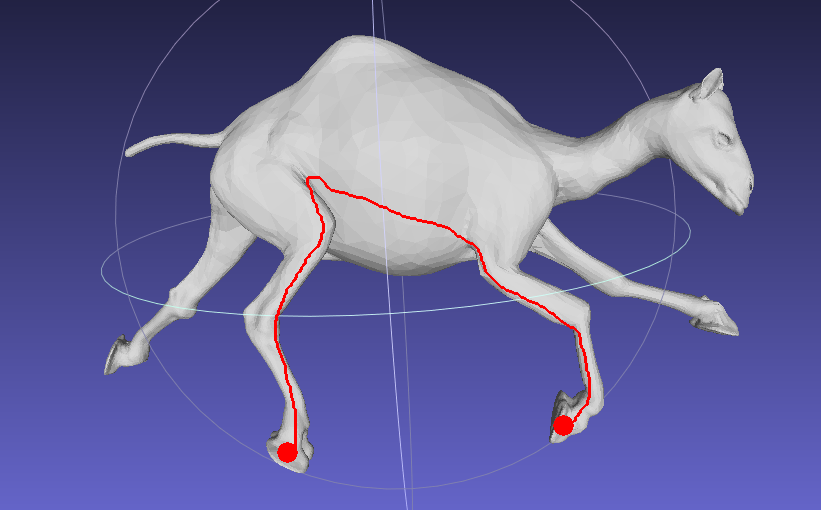
\includegraphics[width=0.35\textwidth]{camel1_geodesic.png}
\end{figure}

\begin{figure}[t]
    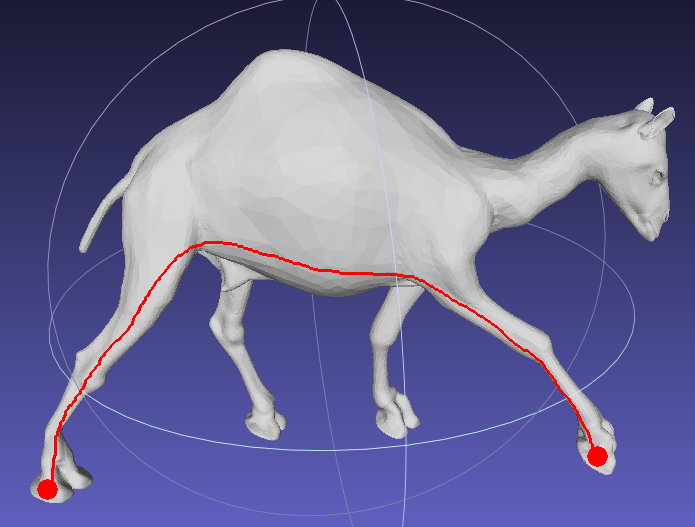
\includegraphics[width=0.32\textwidth]{camel2_geodesic.png}
\end{figure}

\uncover<2->{
What if we try to apply MDS to the distance matrix we get from geodesic distances?
}

\end{frame}


\begin{frame}{Face Example}

\begin{columns}
\begin{column}[T]{5cm}
\begin{figure}[t]
    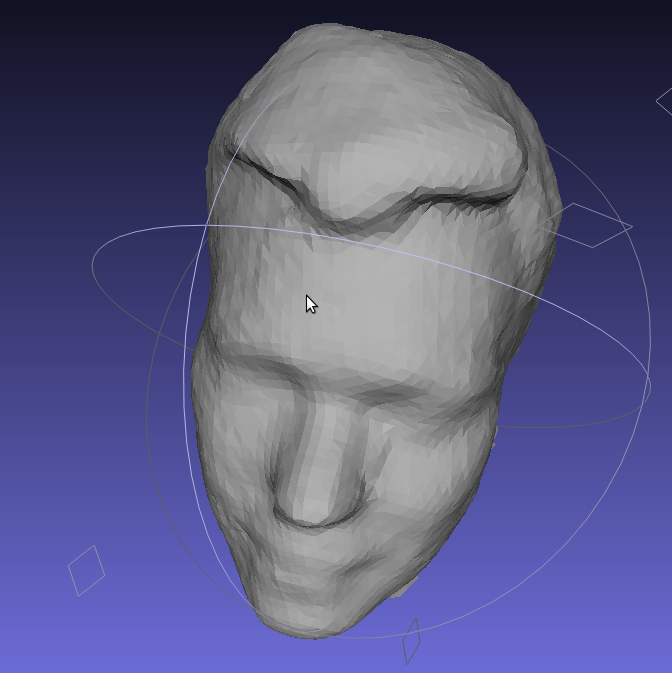
\includegraphics[width=\textwidth]{ChrisOrig.png}
\end{figure}
\end{column}

\begin{column}[T]{5cm}

\uncover<2->{
\begin{figure}[t]
    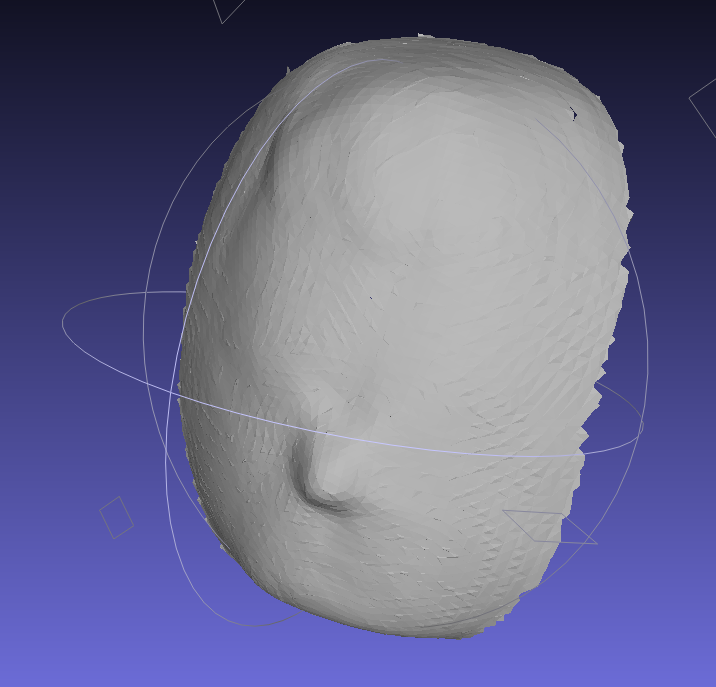
\includegraphics[width=\textwidth]{ChrisCanonical.png}
\end{figure}
}
\end{column}
\end{columns}

\end{frame}


\begin{frame}{Face Example}

\begin{columns}
\begin{column}[T]{5cm}
\begin{figure}[t]
    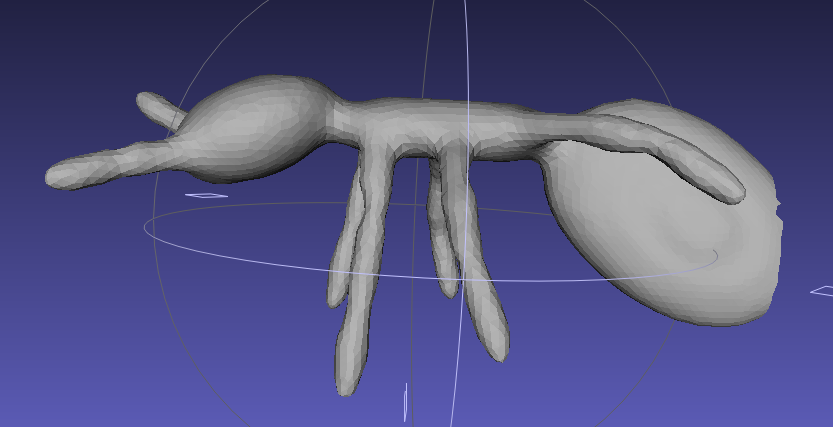
\includegraphics[width=\textwidth]{bug.png}
\end{figure}
\end{column}

\begin{column}[T]{5cm}

\uncover<2->{
\begin{figure}[t]
    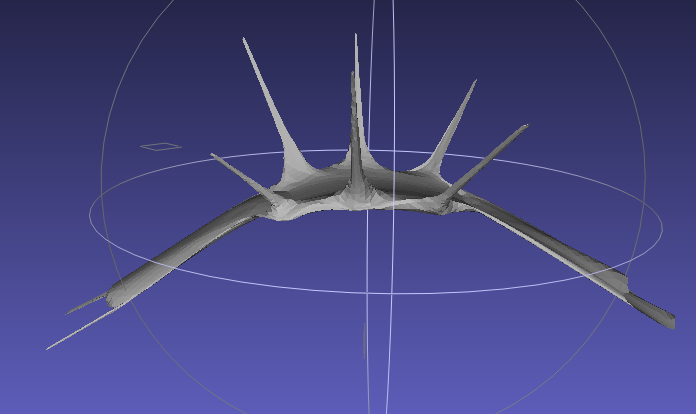
\includegraphics[width=\textwidth]{bugCanonical.png}
\end{figure}
}
\end{column}
\end{columns}

\end{frame}

\begin{frame}{More Examples}

\begin{figure}[t]
    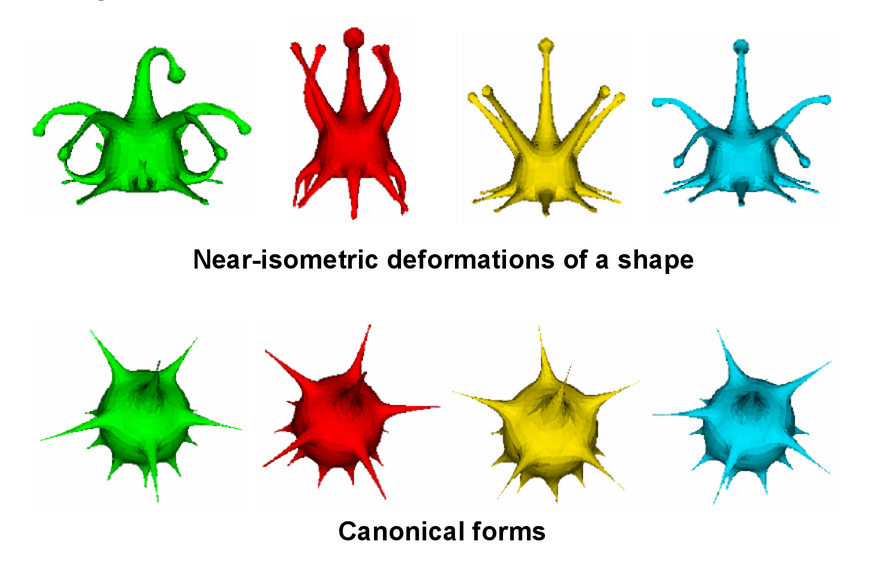
\includegraphics[width=0.8\textwidth]{Bronstein_CanonicalForms.png}
\end{figure}

\textcolor{red}{Bronstein}

\end{frame}

\begin{frame}{Lots More Examples}

\begin{figure}[t]
    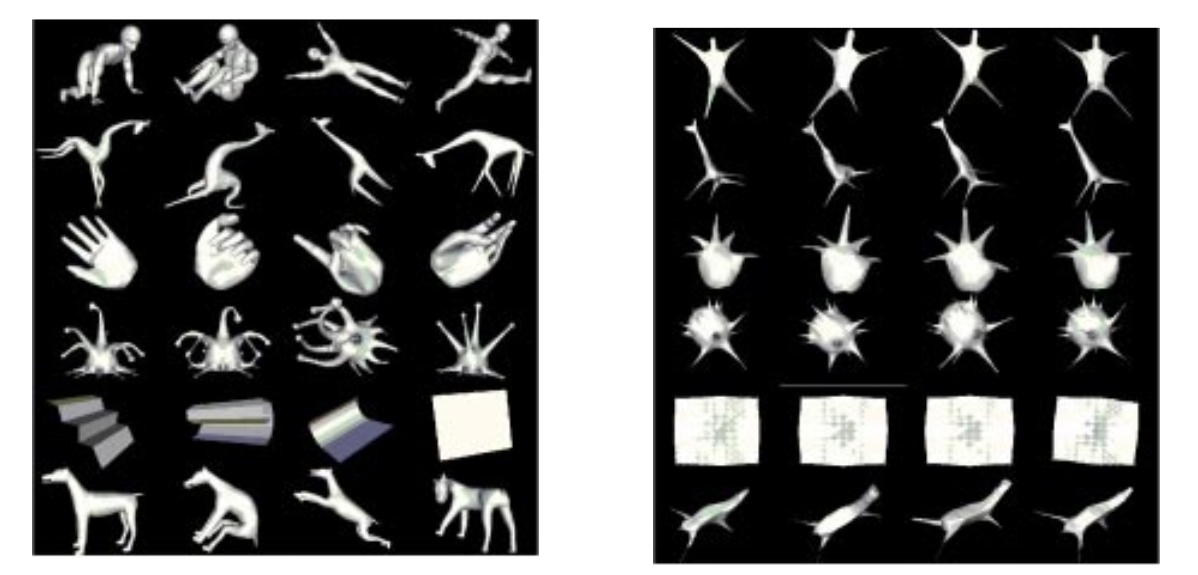
\includegraphics[width=\textwidth]{EladKimmel_CanonicalForms.png}
\end{figure}
\textcolor{red}{Elad Kimmel 2001: ``Bending Invariant Representations for Surfaces''}

\end{frame}


\end{document}

